\chapter{地图符号}

\section{类结构}

\newpage
\pdfpagewidth=420mm
\pdfpageheight=297mm

\thispagestyle{empty}

\begin{center}
	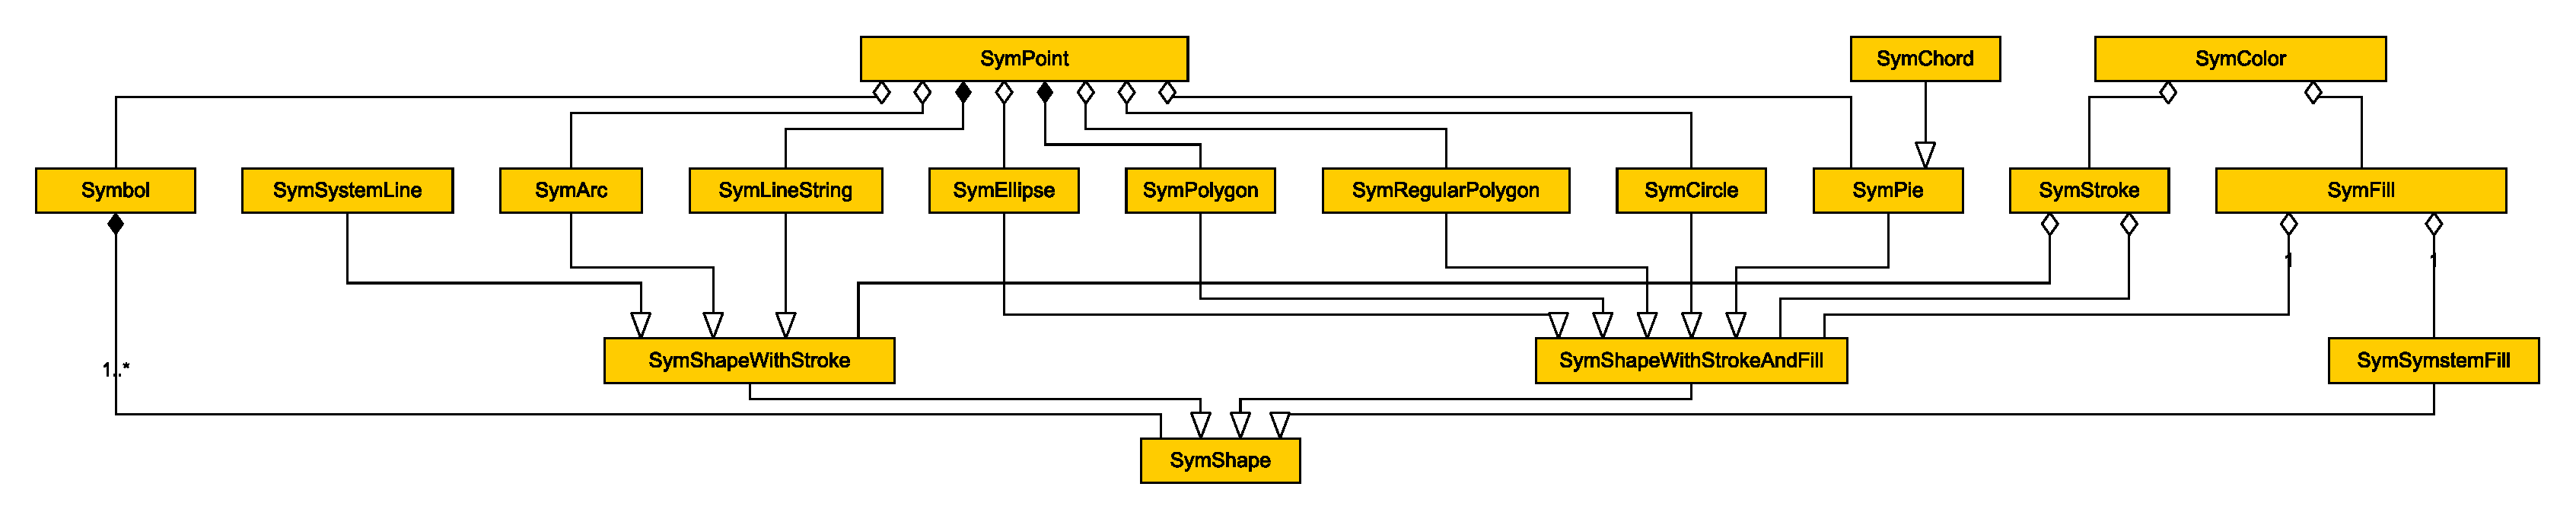
\includegraphics[width=35cm]{Symbol_extension/symbol_class_structure.eps}
\end{center}

%\begin{tikzpicture}[gridded]
%	
%	\begin{class}[text width=3cm]{Symbol}{6,3}
%		
%	\end{class}
%	
%	\begin{class}[text width=3cm]{SymPoint}{0,0}
%		
%	\end{class}
%	
%	
%	\begin{class}[text width=3cm]{SymShape}{15,0}
%		
%	\end{class}
%	
%	\begin{class}[text width=4cm]{SymShapeWithStroke}{4,-2}
%		\inherit{SymShape}
%	\end{class}
%	
%	\begin{class}[text width=6cm]{SymShapeWithStrokeAndFill}{15,-2}
%		\inherit{SymShape}
%	\end{class}
%	
%	\begin{class}[text width=3cm]{SymSystemFill}{25,-2}
%		\inherit{SymShape}
%	\end{class}
%	
%	\begin{class}[text width=3cm]{SymSystemLine}{0,-4}
%		\inherit{SymShapeWithStroke}
%	\end{class}
%	
%	\begin{class}[text width=3cm]{SymArc}{4,-4}
%		\inherit{SymShapeWithStroke}
%	\end{class}
%	
%	\begin{class}[text width=3cm]{SymLineString}{8,-4}
%		\inherit{SymShapeWithStroke}
%	\end{class}
%	
%	
%	\begin{class}[text width=3cm]{SymCircle}{4,-6}
%		\inherit{SymShapeWithStrokeAndFill}
%	\end{class}
%	
%	\begin{class}[text width=3cm]{SymEllipse}{8,-6}
%		\inherit{SymShapeWithStrokeAndFill}
%	\end{class}
%	
%	\begin{class}[text width=3cm]{SymChord}{12,-6}
%		\inherit{SymShapeWithStrokeAndFill}
%	\end{class}
%	
%	\begin{class}[text width=3cm]{SymPie}{16,-6}
%		\inherit{SymShapeWithStrokeAndFill}
%	\end{class}
%	
%	\begin{class}[text width=3cm]{SymPolygon}{20,-6}
%		\inherit{SymShapeWithStrokeAndFill}
%	\end{class}
%	
%	
%	\begin{class}[text width=3cm]{SymRegularPolygon}{24,-6}
%		\inherit{SymShapeWithStrokeAndFill}
%	\end{class}
%	
%	\composition{SymPoint}{}{2..*}{SymLineString}
%	
%%	\begin{class}[text width=4cm]{SymPoint}{30,0}
%%		\attribute{x : double}
%%		\attribute{y : double}
%%	
%%		\operation{from\_json\_object(json\_object*) : bool}	
%%		\operation{to\_json\_object() : json\_object*}
%%		\operation{getErrorMessage() : string}
%%		\operation{memory\_size() : size\_t}
%%		\operation{serialize(const char* ) : char*}
%%		\operation{deserialize(const char*) : char*}
%%	\end{class}
%%	
%%	\begin{class}[text width=6cm]{Symbol}{0,0}
%%		\attribute{offset : SymPoint}
%%		\attribute{xscale : double}
%%		\attribute{yscale : double}	
%%		\operation{from\_json\_file(const char*) : bool}	
%%		\operation{from\_json\_string(const char*) : bool}
%%		\operation{to\_json\_string() : string}
%%		\operation{getErrorMessage() : string}
%%		\operation{clear() : void}
%%		\operation{memory\_size() : size\_t}
%%		\operation{serialize(size\_t\& len) : char*}
%%		\operation{deserialize(const char*) : bool}
%%	\end{class}
%
%	
%\end{tikzpicture}

\newpage
\pdfpagewidth=210mm
\pdfpageheight=297mm